\chapter{Introduzione al corso}

In questo corso si studieranno principalmente servizi e protocolli di rete (TCP/IP, DNS, HTTP, NAT, SSL), in particolare, il focus principale è sul networking ovvero il trasferimento di dati dal dispositivo client al server e viceversa.

\section{Le reti}

\begin{redbar}
Una \textbf{rete} è composta di dispositivi (nodi) in grado di scambiarsi informazioni, quali sistemi terminali (end system), e dispositivi di interconnessione. I sistemi terminali possono essere di due tipi: \textit{host} o \textit{server}. Un host è una macchina in genere di proprietà degli utenti e dedicata ad eseguire applicazioni, quale un computer desktop, un portatile, un cellulare o un tablet. Un server è tipicamente un computer con elevate prestazioni destinato a eseguire programmi che forniscono servizio a diverse applicazioni utente come, per esempio, la posta elettronica o il Web. 
\end{redbar}

I server sono installati in uffici centrali e vengono gestiti dagli amministratori di sistema. Rientrano tra i server anche le periferiche di rete, come per esempio le stampanti, che vengono spesso condivise tra i vari utenti.

I dispositivi di interconnessione rigenerano/modificano il segnale che ricevono e si distinguono in: \textit{router} che sono dispositivi che collegano una rete ad altre reti; \textit{switch} (commutatori) che collegano più sistemi terminali a livello locale; \textit{modem} che trasformano la codifica dei dati.
Tutti questi dispositivi vengono collegati utilizzando mezzi trasmissivi cablati o wireless genericamente chiamati \textit{link} (collegamenti).

I collegamenti cablati possono essere in rame o fibra ottica e un bit viaggia da un sistema terminale a un altro, passando per una serie di coppie trasmittente-ricevente. I mezzi di trasmissione cablati sono: il doppino intrecciato, formato da due fili di rame distinti (tradizionale cavo telefonico) o intrecciato da quattro coppie di fili (Ethernet); il cavo coassiale, formato due conduttori in rame concentrici, usato per cablatura di reti locali ad alta velocità ed è molto resistente alle interferenze; la fibra ottica, è un mezzo sottile e flessibile che conduce impulsi di luce (ciascun impulso rappresenta un bit), ha alta frequenze trasmissiva, elevata velocità di trasmissione punto-punto, basso tasso di errore ed è immune all'interferenza elettromagnetica. Per questi motivo è il mezzo prevalente delle dorsali internet.

Con i mezzi trasmissivi wirless, i segnali si propagano nell'atmosfera e nello spazio esterno. Il vantaggio di questo tipo di sistemi è che trasportano segnali nello spettro elettromagnetico e non richiedono l'installazione fisica di cavi, ma allo stesso tempo possono essere soggetti alla rifrazione, ostruzione da parte di ostacoli o interferenza. I principali tipi di canali radio sono: microonde terrestri, LAN, wide-area e satellitari.

\subsection{LAN (Local Area Network)}
Una LAN (Local Area Network), o rete locale, è solitamente una rete privata che collega i sistemi terminali in un singolo ufficio (azienda, università) e non specifica un numero minimo o massimo di dispostivi. Ogni sistema terminale nella LAN ha un indirizzo che lo identifica univocamente nella rete. 

In passato tutti i dispositivi di una rete locale erano collegati mediante un cavo condiviso, o mezzo broadcast, per cui il pacchetto inviato da un dispositivo veniva ricevuto da tutti. Il destinatario elaborava il pacchetto, mentre gli altri lo dovevano ignorare. Oggi la maggior parte delle LAN utilizza uno switch di interconnessione, al quale ogni dispositivo in rete è direttamente connesso. Lo switch è in grado di riconoscere l'indirizzo di destinazione e di inviare il pacchetto al solo destinatario senza inviarlo agli altri dispositivi. Lo switch riduce il traffico nella LAN e consente a più coppie di dispositivi di comunicare contemporaneamente fra di loro, posto che non vi siano dispositivi sorgente o destinazione in comune.

\begin{figure}[ht]
    \centering
    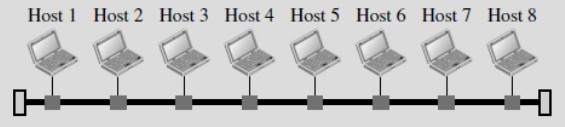
\includegraphics[width=8.5cm]{images/LAN-brodcast.PNG}
    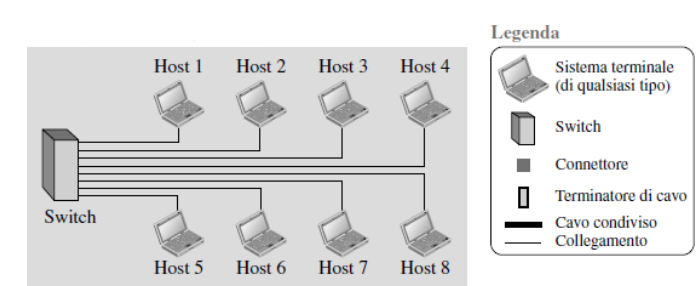
\includegraphics[width=9cm]{images/LAN-switch.PNG}
    \caption{LAN con cavo condiviso e con switch}
    \label{fig:brodcast-switch}
\end{figure}

\subsection{WAN (Wide Area Network)}
Anche una WAN (Wide Area Network), o rete geografica, è un'interconnessione di dispositivi in grado di comunicare, ma esistono notevoli differenze rispetto alle LAN. Queste ultime sono solitamente di estensione limitata, mentre una WAN ha un'estensione decisamente superiore, potendo servire una città, una regione, una nazione o addirittura l'intero globo. Una LAN interconnette prevalentemente sistemi terminali, mentre una WAN interconnette anche switch, router o modem. Una LAN è solitamente di proprietà dell'organizzazione che la utilizza, mentre una WAN è generalmente creata e gestita da un operatore di telecomunicazioni, Internet Service Provider (ISP), che fornisce i suoi servizi alle organizzazioni che ne fanno uso. Oggi esistono due tipi di WAN: punto-punto e a commutazione (switched).
\begin{itemize}
    \item Una WAN punto-punto è una rete che collega due dispositivi di comunicazione tramite un mezzo trasmissivo (cavo o wireless);
    \item Una WAN a commutazione (switched) è una rete con più di due punti di terminazione e viene utilizzata nelle dorsali dell'odierna rete globale.
\end{itemize}

\begin{figure}[ht]
    \centering
    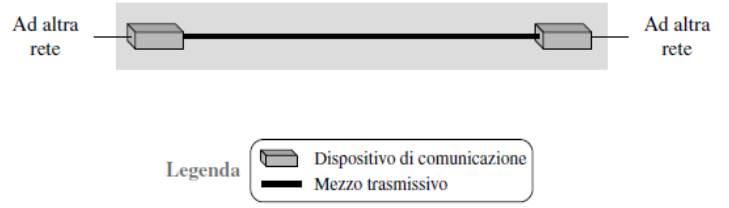
\includegraphics[width=8cm]{images/WAN-punto-punto.PNG}
    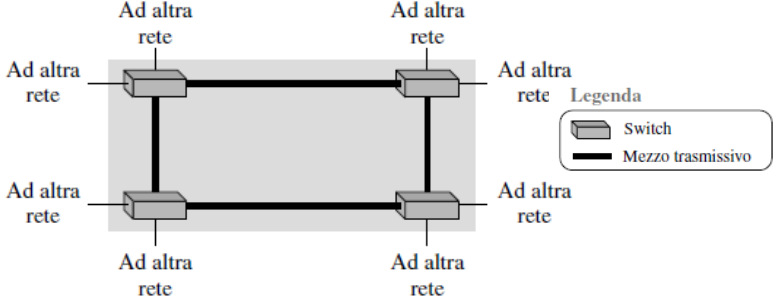
\includegraphics[width=7cm]{images/WAN-commutazione.PNG}
    \caption{WAN punto-punto e WAN a commutazione}
    \label{fig:ptpt-comm-inter}
\end{figure}

Al giorno d'oggi è raro vedere LAN o WAN isolate: esse sono in genere connesse fra di loro, formando una internetwork, o internet. 

\begin{Example}{Internetwork}{}
    S\textit{i ipotizzi che un'azienda abbia due uffici in città di regioni differenti, Roma e Bologna. In ciascun ufficio esiste una LAN che consente agli impiegati di comunicare l'uno con l'altro. Per rendere possibile la comunicazione fra gli impiegati di uffici differenti, l'azienda affitta un'apposita WAN punto-punto da un ISP, per esempio una compagnia telefonica, per collegare le due LAN. A questo punto l'azienda ha realizzato una internetwork, o una rete internet privata, che consente la comunicazione fra le due reti.}

    \begin{minipage}{\textwidth}
        \centering
        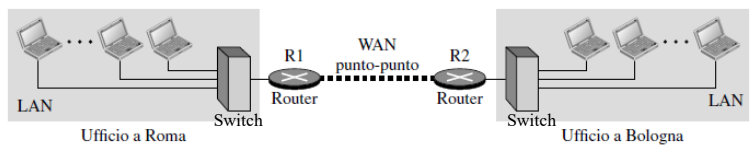
\includegraphics[width=0.8\linewidth]{images/internetwork.PNG}
        %\captionof{figure}{Esempio}
    \end{minipage}
    
    Quando un host in un ufficio invia un messaggio a un altro host nello stesso ufficio, lo switch trasmette il messaggio all'host indirizzato. Quando invece un host nell'ufficio di Roma invia un messaggio a un host nell'ufficio di Bologna, è il router R1 che instrada il pacchetto al router R2 per raggiungere il destinatario.
\end{Example}

\begin{figure}[ht]
    \centering
    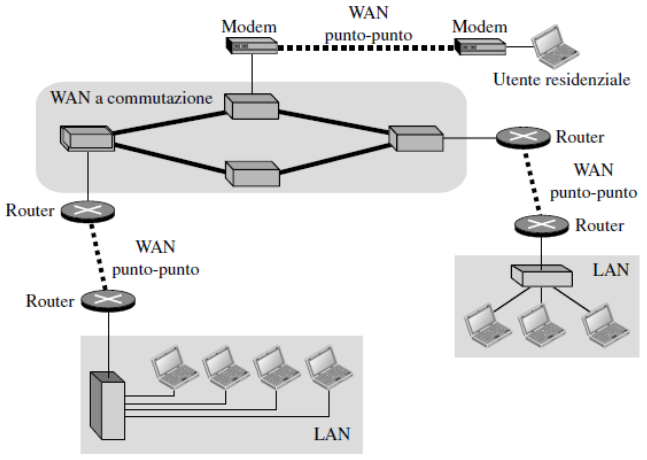
\includegraphics[width=10cm]{images/rete-eterogenea-LAN-WAN.PNG}
    \caption{Rete eterogenea composta da quattro WAN e tre LAN}
    \label{fig:rete-eterogenea}
\end{figure}

La rete GARR (Gruppo per l'Armonizzazione delle Reti della Ricerca) interconnette ad altissima capacità università, centri di ricerca, biblioteche, musei, scuole e altri luoghi in cui si fa istruzione, scienza, cultura e innovazione su tutto il territorio nazionale. E' un'infrastruttura in fibra ottica che utilizza le più avanzate tecnologie di comunicazione e si sviluppa su circa 15.000 km tra collegamenti di dorsale e di accesso. Oggi la capacità delle singole tratte della dorsale arriva a 100 Gbps, mentre quella dei collegamenti di accesso può raggiungere i 40 Gbps in base alle necessità di banda della sede. Grazie alla grande scalabilità delle tecnologie utilizzate, queste capacità possono evolvere facilmente insieme alle necessità degli utenti.


\section{Commutazione (Switching)}
Si è affermato che una internet è una combinazione di link e dispositivi capaci di scambiarsi informazioni. In particolare i sistemi terminali appartenenti alla rete comunicano tra di loro per mezzo di dispositivi come switch e router che si trovano nel percorso (o rotta) tra il sistema sorgente e destinazione. In base al metodo adottato per determinare il percorso tra due sistemi terminali in comunicazione si possono distinguere due tipi di reti: a commutazione di circuito e a commutazione di pacchetto.

\subsection{Reti a commutazione di circuito}
In una rete a commutazione di circuito (circuit-switched network) tra due dispositivi è sempre disponibile un collegamento dedicato, chiamato circuito; lo switch che collega i due dispositivi può solo attivarlo o disattivarlo. Le risorse necessarie al circuito sono riservate per l'intera durata della comunicazione e le informazioni riguardanti il circuito vengono mantenute dalla rete. Anche se esistono più percorsi tra due dispositivi in comunicazione, solo uno di questi verrà usato per l'intera comunicazione e comunicazioni diverse tra gli stessi dispositivi possono usare circuiti stabiliti su percorsi diversi.

\begin{Example}{Reti a commutazione di circuito}{}
    \textit{Quattro apparecchi telefonici su ciascun lato sono collegati a uno switch che mette in comunicazione un apparecchio telefonico da un lato con un apparecchio telefonico dall'altro lato. La linea tra i due switch è una linea di comunicazione a elevata capacità che può gestire contemporaneamente quattro canali voce; tale capacità può essere condivisa fra tutte le coppie di apparecchi telefonici. Gli switch impiegati in questo esempio sono in grado di inoltrare informazioni ma non di memorizzarle.}

    \begin{minipage}{\textwidth}
        \centering
        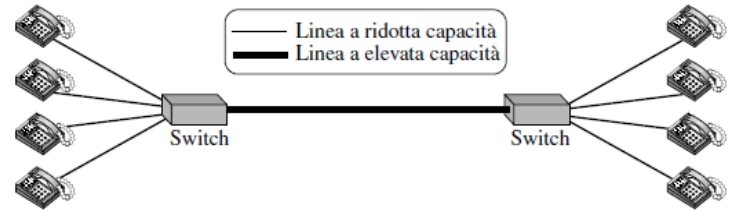
\includegraphics[width=0.7\linewidth]{images/esempio-comm-circuito.PNG}
        %\captionof{figure}{Esempio}
    \end{minipage}
    
    Si prendano ora in considerazione le due situazioni seguenti. Nella prima tutti gli apparecchi telefonici sono occupati: quattro persone da un lato sono in comunicazione con le quattro persone all'altro lato e la capacità della linea è completamente utilizzata. Nella seconda situazione solo un apparecchio telefonico da un lato è collegato a un apparecchio telefonico dell'altro lato: si impiega dunque solamente un quarto della capacità della linea. Questo comporta che una rete a commutazione di circuito risulta efficiente solamente quando è utilizzata alla sua massima capacità, mentre nella maggior parte del tempo è inefficiente perché sottoutilizzata.
\end{Example}

In questo tipo di rete le risorse (ad es. ampiezza di banda - bandwidth) vengono suddivise in "pezzi" per frequenza o per tempo, e ciascun “pezzo” viene allocato ai vari collegamenti.

\subsection{Reti a commutazione di pacchetto}
In questa rete di computer la comunicazione fra i due lati viene effettuata trasmettendo blocchi di dati chiamati pacchetti. Invece di avere una comunicazione continua, i due dispositivi comunicano scambiandosi pacchetti di dati. Gli switch sono in grado di memorizzare i pacchetti (store), oltre che di inoltrarli (forward), essendo i pacchetti entità indipendenti che possono essere memorizzate e inviate successivamente. Non c'è un percorso specifico che viene usato per il trasferimento di dati tra due dispositivi: blocchi di dati, anche dello stesso file o comunicazione, possono prendere percorsi diversi nel viaggio dalla sorgente alla destinazione e arrivare a destinazione in un ordine diverso.

\begin{Example}{Reti a commutazione di pacchetto}{}
    \textit{Un router in una rete a commutazione di pacchetto possiede una coda dove possono essere memorizzati i pacchetti prima di essere inoltrati. Si ipotizzi che la capacità della linea di comunicazione fra i due router sia solo il doppio della capacità delle linee dei dati che collegano i computer ai router.} 
    
    \begin{minipage}{\textwidth}
        \centering
        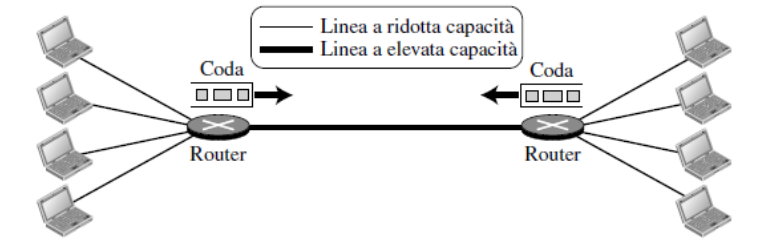
\includegraphics[width=0.7\linewidth]{images/esempio-comm-pacc.PNG}
        %\captionof{figure}{Esempio}
    \end{minipage}
    
    Nel caso in cui due soli computer, uno per ciascun lato, dovessero comunicare fra di loro, non vi sarebbe alcun tempo di attesa per i pacchetti, che verrebbero inoltrati appena disponibili. Se invece i pacchetti arrivassero a un router quando la linea di comunicazione fra i due router fosse già utilizzata alla sua massima capacità, i pacchetti dovrebbero essere memorizzati per essere successivamente inoltrati nell'ordine di arrivo. 
\end{Example}

Questo esempio dimostra che una rete a commutazione di pacchetto è più efficiente di una rete a commutazione di circuito, ma che i pacchetti potrebbero incorrere in qualche ritardo.

\section{Internet}

\begin{Notation}{Internet}{}
    internet (con la i minuscola) rappresenta due o più reti interconnesse. L'internet più famosa è chiamata Internet (I maiuscola) ed è composta da migliaia di reti interconnesse.
\end{Notation}

\begin{figure}[ht]
    \centering
    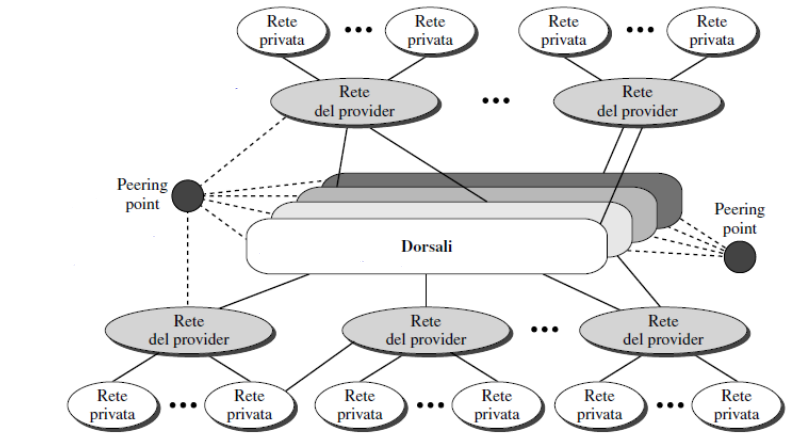
\includegraphics[width=11cm]{images/rapp-conc-internet.PNG}
    \caption{Rappresentazione concettuale di Internet}
    \label{fig:rapp-conc-internet}
\end{figure}

La figura \ref{fig:rapp-conc-internet} rappresenta Internet come un insieme di dorsali (backbone), reti dei provider e reti private. Al livello più elevato le dorsali sono reti particolarmente estese di proprietà di qualche compagnia telefonica. Queste reti dorsali sono interconnesse tramite sistemi di commutazione notevolmente complessi, chiamati peering point. Al secondo livello vi sono reti più piccole, chiamate reti dei provider, che utilizzano a pagamento i servizi delle dorsali. Le reti dei provider sono connesse alle dorsali e a volte ad altre reti di provider. Le reti private sono reti ai confini di Internet (last hop network), più vicine ai sistemi terminali, che utilizzano i servizi a pagamento forniti dalle reti dei provider.

Le dorsali e le reti dei provider sono anche chiamate collettivamente ISP (Internet Service Provider). Le dorsali sono spesso chiamate ISP internazionali, le reti dei provider ISP nazionali o regionali.

\section{L'accesso a Internet}
Internet è una internetwork che consente a qualsiasi utente di farne parte. L'utente, tuttavia, deve essere fisicamente collegato a un ISP, solitamente mediante una WAN punto-punto. Il collegamento che connette l'utente al primo router di Internet è detto rete di accesso.

\subsection{Accesso via rete telefonica}
Oggi la maggior parte delle abitazioni e delle piccole aziende è dotata di servizi telefonici, quindi è collegata a una rete telefonica. Poiché molte reti telefoniche sono collegate a Internet, un'opzione è quella di collegarsi a Internet modificando la linea telefonica fra la sede del dispositivo che vuole connettersi e la centrale telefonica con una WAN punto-punto. Questo può avvenire in due modi.

\begin{enumerate}
    \item \textit{Servizio dial-up.} Questa soluzione consiste nell'inserire sulla linea telefonica un modem che converte i dati digitali (del computer) in analogici (per trasmetterli sulla linea telefonica) e viceversa. Sfortunatamente il servizio dial-up è molto lento; inoltre, quando la linea è utilizzata per il collegamento a Internet non può essere utilizzata per le normali conversazioni telefoniche (vocali). Si tratta quindi di una soluzione adatta a clienti residenziali o a piccole aziende che si connettono a Internet solo sporadicamente.
    \item \textit{Servizio DSL (Digital Subscriber Line).} Negli ultimi anni numerose compagnie telefoniche hanno modificato le proprie linee telefoniche per poter fornire ai clienti residenziali e alle piccole imprese servizi di accesso a Internet ad alta velocità. La tecnologia DSL supporta la comunicazione digitale ad alta velocità sulla linea telefonica. Questo servizio consente anche di utilizzare simultaneamente la linea telefonica per il traffico dati e per le comunicazioni vocali.
\end{enumerate}

\subsection{Accesso tramite Ethernet}
Nelle reti aziendali e universitarie la tecnologia usata per l'accesso a Internet è l'Ethernet dove lo switch (Ethernet) della LAN è generalmente collegato a un router istituzionale che è connesso ai router della dorsale.

\subsection{Accesso wireless}
La connettività wireless si è ampiamente diffusa. Con il continuo sviluppo di tecnologie di accesso wireless, i clienti residenziali e le piccole aziende possono convenientemente utilizzare un'opportuna combinazione di collegamenti wireless e via cavo per accedere a Internet. Esempi di accessi wireless sono: Wi-Fi con access point (locale) connesso alla Ethernet cablata e raggio di azione di qualche decina di metri oppure cellulare, dove si usa la rete cellulare con access point (base station) della compagnia telefonica cellulare, con raggio di azioni di decine di kilometri.

\section{Capacità e prestazioni delle reti}
Un argomento di cui si parla spesso nell'ambito delle reti è la velocità della rete o di un collegamento, ovvero quanto velocemente si riesce a trasmettere e ricevere i dati. In realtà, il concetto di velocità è molto ampio e coinvolge vari fattori che influiscono sulle prestazioni (performance) di una rete.
Nel caso di una rete a commutazione di pacchetto, le metriche che ne determinano le prestazioni si misurano in termini di: ampiezza di banda, bit rate, throughput, ritardi e perdita di pacchetti.

\subsection{Ampiezza di banda e bit rate}
Con il termine ampiezza di banda si indicano due concetti leggermente diversi ma strettamente legati. 
\begin{enumerate}
    \item Al livello di caratterizzazione di un canale o di un sistema trasmissivo, l'ampiezza di banda (bandwidth), o banda, è una quantità che si misura in hertz e rappresenta la larghezza dell'intervallo di frequenze utilizzato dal sistema trasmissivo, ovvero l'intervallo di frequenze che un mezzo fisico consente di trasmettere senza danneggiare il segnale in maniera irrecuperabile. In generale, maggiore è l'ampiezza di banda, maggiore è la quantità di informazione che può essere veicolata attraverso il mezzo trasmissivo.
    \item Quando viene espressa in bit al secondo (bps), la banda rappresenta invece il bit o transmission rate (velocità di trasmissione), per brevità rate, ovvero la quantità di bit al secondo che un certo link garantisce di trasmettere.
\end{enumerate}

I due concetti sono legati ma non coincidenti, in quanto il bit rate di un link dipende sia dalla banda (in hertz) che dalla specifica tecnica di trasmissione, o formato di modulazione digitale utilizzato. In generale, il bit rate è proporzionale alla banda in hertz. Infine, per banda di un tipo di rete, si intende il bit rate garantito (nominalmente) dai suoi link. Per esempio si può dire che il rate di un link Fast Ethernet è di 100 Mbps. Ciò significa che tale rete può inviare al massimo 100 Mbps. Il rate fornisce quindi un'indicazione della capacità della rete di trasferire dati.

\subsection{Throughput}
Il throughput indica quanto velocemente riusciamo effettivamente a inviare i dati tramite una rete. Sebbene a prima vista il rate e il throughput sembrino la stessa cosa, in realtà non lo sono. Un link può avere un rate di $B$ bps, ma possiamo inviare solo $T$ bps tramite quel link, con $T$ sempre inferiore a $B$. In altre parole, il rate è una misura della potenziale velocità di un link; il throughput è una misura dell'effettiva velocità di un link (quanto velocemente riusciamo a inviare i dati in realtà). Per esempio, possiamo avere un link con un rate di 1 Mbps, ma i dispositivi connessi alle estremità del link possono gestire solamente 200 kpbs. Ciò significa che non possiamo inviare più di 200 kbps attraverso quel link.

Immaginiamo un'autostrada progettata per far transitare 1000 auto al minuto da un punto a un altro. Tuttavia, se c'è traffico sulla strada, tale cifra può essere ridotta a 100 auto al minuto. Il rate è 1000 auto al minuto, il throughput 100 auto al minuto.

E' importante notare che il throughput è definito come il numero dei bit che passano attraverso un punto della rete in un secondo. In un percorso da una sorgente a una destinazione un pacchetto può passare attraverso numerosi link, ognuno con un throughput diverso. Come possiamo allora determinare il throughput dell'intero percorso? 

\begin{Example}{Throughput}{}
    \textit{Supponiamo di avere tre link, come mostrato in figura:}

    \begin{minipage}{\textwidth}
        \centering
        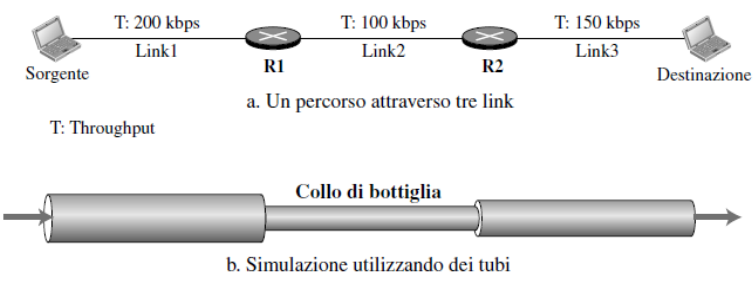
\includegraphics[width=0.7\linewidth]{images/esempio-throughput.PNG}
        %\captionof{figure}{Esempio}
    \end{minipage}
    
    I dati possono scorrere alla velocità di 200 kbps nel link 1. Tuttavia, quando i dati arrivano al router R1, non possono passare alla stessa velocità. I dati devono essere accodati al router e inviati a 100 kbps. Quando i dati arrivano al router R2, potrebbero essere inviati alla velocità di 150 kbps ma non ci sono sufficienti dati da inviare. In altre parole, la velocità media del flusso di dati nel link 3 è anch'essa di 100 kbps. Possiamo concludere che il throughput dei dati per questo percorso è di 100 kbps, la minore delle tre diverse velocità dei dati. La figura mostra anche che possiamo simulare il comportamento in ogni link con tubi di diverse dimensioni; il throughput medio è determinato dal collo di bottiglia, il tubo con il diametro minore.
\end{Example}

In generale in un percorso con $n$ link in serie abbiamo:
\begin{equation*}
    Throughput = minimo(T_1, T_2,... T_n)
\end{equation*}

Anche se l'esempio illustrato mostra come calcolare il throughput quando i dati passano attraverso numerosi link, la situazione reale in Internet è che i dati normalmente passano attraverso due reti di accesso e la dorsale di Internet, come mostrato nella Figura \ref{fig:throughput}.

\begin{figure}[ht]
    \centering
    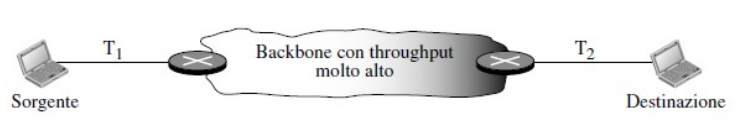
\includegraphics[width=11cm]{images/throughput.PNG}
    \caption{Throughput attraverso il backbone di Internet}
    \label{fig:throughput}
\end{figure}

La dorsale di Internet ha un throughput molto alto, nell'ordine di gigabit al secondo. Ciò significa che il throughput normalmente viene definito come il minimo tra i due link d'accesso che collegano la sorgente e la destinazione alla dorsale. La Figura \ref{fig:throughput} illustra tale situazione, in cui il throughput è il minimo di $T_1$ e $T_2$. Ad esempio, se un server connesso ad Internet tramite una Fast Ethernet LAN con la velocità dei dati di 100 Mbps, ma un utente che vuole scaricare un file collegato ad Internet tramite una linea telefonica commutata con velocità di dati di 40 kbps, il throughput è di 40 kbps. Il collo di bottiglia è certamente la linea commutata.

Dobbiamo parlare di un'altra situazione nella quale pensiamo al throughput. Il link tra due router non è sempre dedicato ad un flusso. Un router può raccogliere il flusso da varie sorgenti o distribuirlo tra diverse sorgenti. In questo caso il rate del link tra i due router è realmente condiviso tra i flussi e ciò va considerato quando si calcola il throughput. Per esempio, nella Figura \ref{fig:throughput2} la velocità del link principale nel calcolo del throughput è solo 200 kbps in quanto il link viene condiviso tra tre percorsi.

\begin{figure}[ht]
    \centering
    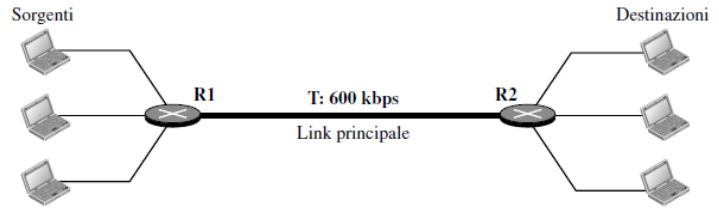
\includegraphics[width=10cm]{images/throughput2.PNG}
    \caption{Effetto del throughput nei link condivisi}
    \label{fig:throughput2}
\end{figure}

\subsection{Latenza (ritardo)}
Tutti noi ci aspettiamo risposte istantanee da una rete, ma un pacchetto che viaggia dalla sorgente alla destinazione accumula dei ritardi. La latenza, o ritardo (delay), definisce quanto tempo serve affinché un intero messaggio arrivi completamente a destinazione dal momento in cui il primo bit parte dalla sorgente. I ritardi si possono dividere in quattro tipi: ritardo di trasmissione, ritardo di propagazione, ritardo di elaborazione e ritardo di accodamento. La latenza, o ritardo totale, deriva dalla seguente formula:
\begin{align*}
    Latenza = {\text{\textit{ritardo di propagazione}}} + {\text{\textit{ritardo di trasmissione}}} \\+ {\text{\textit{ritardo di accodamento}}} + {\text{\textit{ritardo di elaborazione}}}
\end{align*}

Analizziamo ora i vari tipi di ritardo.

\subsubsection*{Ritardo di trasmissione}
Quando un dispositivo sorgente invia un pacchetto, esso deve immettere sulla linea di trasmissione (ovvero trasmettere) i bit del pacchetto uno per uno. I pacchetti vengono trasmessi in first-come-first-served e se il primo bit del pacchetto viene trasmesso al tempo $t_1$, e l'ultimo bit viene messo in linea al tempo $t_2$ il ritardo di trasmissione del pacchetto è $(t_2 - t_1)$. Chiaramente il ritardo di trasmissione è maggiore per un pacchetto più lungo e minore se il mittente riesce a trasmettere più velocemente. In altre parole il ritardo di trasmissione è:
\begin{equation*}
    Ritardo_{tr} = (\text{\textit{Lunghezza del pacchetto}}) / (Rate)
\end{equation*}

Per esempio in una Fast Ethernet LAN con un rate di 100 milioni di bit al secondo e un pacchetto di 10.000 bit, servono $(10.000)/(100.000.000)$ o 100 microsecondi affinché tutti i bit del pacchetto vengano trasmessi.

\subsubsection*{Ritardo di propagazione}
Il ritardo di propagazione è il tempo che serve ad un bit per viaggiare dal punto A al punto B nel mezzo di trasmissione. Il ritardo di propagazione dipende dalla velocità di propagazione del mezzo, tipicamente data dalla velocità della luce ($3*10^8 m/s$ nell'etere, $2*10^8 m/s$ nel rame). Il ritardo di propagazione dipende anche dalla distanza tra sorgente e destinazione, ovvero dalla lunghezza del link. In altre parole il ritardo di propagazione è:

\begin{equation*}
    Ritardo_{pr} = (Distanza) / (\text{\textit{Velocità di propagazione}})
\end{equation*}

Per esempio se la lunghezza di un collegamento in una WAN punto-punto è 2.000 metri e la velocità di propagazione dei bit nel cavo è $2*10^8 m/s$, allora il ritardo di propagazione è 10 microsecondi.

\subsubsection*{Ritardo di elaborazione}
Il ritardo di elaborazione è il tempo che serve a un router o a un sistema terminale per ricevere un pacchetto dalla sua porta di input, rimuovere l'intestazione del pacchetto, eseguire una procedura di rilevamento errori e consegnare il pacchetto alla porta di output (nel caso di un router) o al protocollo del livello superiore (nel caso di un sistema terminale).

\subsubsection{Ritardo di accodamento}
Il ritardo di accodamento è tipico dei router. Come analizzeremo meglio in seguito, un router ha una coda di input collegata ad ognuna delle sue porte di ingresso per memorizzare i pacchetti in attesa di elaborazione; il router ha anche una coda di output collegata ad ognuna delle sue porte di uscita per memorizzare i pacchetti in attesa di trasmissione. Il ritardo di accodamento per un pacchetto si misura come il tempo in cui il pacchetto attende nella coda di input e in quella di output di un router. Possiamo paragonare la situazione ad un aeroporto trafficato. Alcuni aerei dovranno attendere l'autorizzazione d'atterraggio (ritardo di input); altri aspetteranno l'autorizzazione al decollo (ritardo di output).

Questo tipo di ritardo può variare da pacchetto a pacchetto, fa uso di misure statistiche e dipende dal tasso di arrivo, dal rate, e dalla lunghezza dei pacchetti. Si definisce intensità di traffico come:
\begin{equation*}
    \text{\textit{Intensità di traffico}} = \frac{\text{\textit{Lunghezza del pacchetto }} x \text{\textit{ Tasso medio di arrivo dei pacchetti}}}{\text{\textit{Rate di trasmissione}}}
\end{equation*}

Se l'intensità di traffico è $\sim 0$ allora ci sarà poco ritardo; se $\to 1$ il ritardo si fa consistente; se è $>1$ si ha più lavoro in arrivo di quanto può essere svolto, con conseguente ritardo medio infinito.

\begin{Example}{Casello autostradale}{}
    \textit{a) Le automobili viaggiano (ossia “si propagano”) alla velocità di 100 km/h. Il casello serve (ossia “trasmette”) un’auto ogni 12 secondi (rate). Quanto tempo occorre perché le 10 auto in carovana abbiano superato il secondo casello? b) Le auto ora “si propagano” alla velocità di 1000 km/h. Al casello adesso occorre 1 min per servire ciascuna auto. Le prime auto arriveranno al secondo casello prima che le ultime auto della colonna lascino il primo?}

     \begin{minipage}{\textwidth}
        \centering
        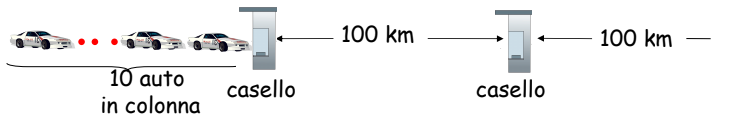
\includegraphics[width=0.8\linewidth]{images/esempio-casello-autostradale.PNG}
        %\captionof{figure}{Esempio}
    \end{minipage}

    \begin{enumerate}[label=(\alph*)]
        \item Il tempo richiesto al casello per trasmettere l’intera colonna sull’autostrada è $10/(5auto/min)= 2 min$ (equivale al tempo di trasmissione). Il tempo richiesto a un’auto per viaggiare dall’uscita di un casello fino al casello successivo è $100km/(100km/h)= 1 hr$ (corrisponde al tempo di propagazione). Il tempo che  intercorre da quando l’intera colonna di vetture si trova di fronte al casello di partenza fino al momento in cui raggiunge quello successivo è la somma del ritardo di trasmissione e del ritardo di propagazione, ovvero 62 minuti.

        \item Si! Dopo 7 minuti, la prima auto sarà al secondo casello, e tre auto saranno ancora in coda davanti al primo casello.
    \end{enumerate}
\end{Example}

\subsubsection*{Prodotto rate-ritardo}
Il rate e il ritardo sono due metriche delle prestazioni di un link. Tuttavia, ciò che è realmente importante nella comunicazione dei dati è il loro prodotto.

Supponiamo di avere un link con rate di 1 bps e un ritardo di 5 secondi. Cosa rappresenta il prodotto rate-ritardo?
Osservando la Figura \ref{fig:prod-rate-ritardo}, possiamo vedere che il prodotto rate-ritardo (1 x 5) è il numero massimo di bit che il link può contenere. Non possono esserci più di 5 bit per volta sul link.

\begin{figure}[ht]
    \centering
    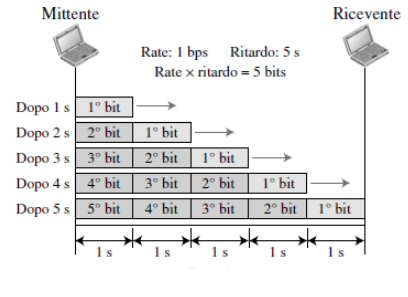
\includegraphics[width=8cm]{images/esempio-prod-rate-ritardo.PNG}
    \caption{Prodotto rate ritardo}
    \label{fig:prod-rate-ritardo}
\end{figure}

Possiamo pensare al link tra due punti come a un tubo. La sezione trasversale del tubo rappresenta il rate e la lunghezza rappresenta il ritardo. Possiamo dire che il volume del tubo definisce il prodotto rate-ritardo.

\subsection{Perdita di pacchetti}
Un'altra questione che influisce gravemente sulle prestazioni della comunicazione è il numero di pacchetti persi durante la trasmissione. Quando un router riceve un pacchetto mentre ne sta elaborando un altro, il pacchetto ricevuto deve essere memorizzato nel buffer di input in attesa del suo turno. Un router tuttavia ha un buffer di input di dimensioni limitate. Può arrivare il momento in cui il buffer è pieno e il pacchetto successivo deve essere saltato. L'effetto della perdita del pacchetto è che deve essere inviato nuovamente dal nodo precedente o dal sistema terminale che lo ha generato, il che a sua volta può creare un'eccedenza di dati e causare la perdita di altri pacchetti, oppure non essere ritrasmesso affatto.

\textit{Ma cosa significano effettivamente packet delay e packet loss nella “vera” Internet?} Una traceroute (tracert) è un programma diagnostico che fornisce una misura del ritardo dalla sorgente a tutti i router lungo il percorso Internet punto-punto verso la destinazione. Per fare questo invia gruppi di tre pacchetti, ogni gruppo con tempo di vita incrementale (da 1 a $n$, $\textit{massimo valore} = 30$) che raggiungeranno il router $i$ ($i=1,...,n$) sul percorso verso la destinazione. Il router $i$ restituirà i pacchetti al mittente e il mittente calcola l’intervallo tra trasmissione e risposta.

L’output del comando \verb|traceroute| presenta 6 colonne: il numero di router sulla rotta; il nome del router; l'indirizzo del router; il tempo di andata e ritorno 1$^\text{o}$ pacchetto; il tempo di andata e ritorno 2$^\text{o}$ pacchetto; il tempo di andata e ritorno 3$^\text{o}$ pacchetto. Il tempo di andata e ritorno (round trip time - RTT) include i 4 ritardi visti precedentemente. 
Può accadere (se c’è congestione o se si segue un percorso diverso) che il RTT del router $n$ sia maggiore del RTT del router $n+1$ a causa dei ritardi di accodamento. Se la sorgente non riceve risposta da un router intermedio (o ne riceve meno di 3) allora pone un asterisco al posto del tempo RTT.

\section{Hardware e software}

Si è fornita una panoramica della struttura e delle prestazioni di Internet, che è costituita da numerose reti di varie dimensioni interconnesse tramite opportuni dispositivi di comunicazione. Tuttavia per poter comunicare non è sufficiente assicurare questi collegamenti, ma è necessario utilizzare sia dell'hardware che del software. Nel capitolo successivo si descriverà come l'hardware e il software vengano coordinati tramite l'impiego di protocolli organizzati in livelli (layer).